\section{Raspberry Pi - Gateway de borda (item 2c)}

\subsection{Função e organização do software}

O Gateway é um serviço Python sem interface gráfica que roda na Raspberry Pi (Raspberry Pi OS, Linux ARM64) e faz a ponte entre a porta serial do CLP e a rede IP. Cada responsabilidade é executada em uma \textit{thread} própria, iniciada e encerrada pela classe \cod{GatewayApplication} (Tabela \ref{tab:gwmodulos}).

{\footnotesize
\begin{longtable}{|>{\raggedright\arraybackslash}p{3.6cm}|>{\raggedright\arraybackslash}p{11.0cm}|}
\caption{Módulos do pacote \cod{hardware/gateway/}.}\label{tab:gwmodulos}\\
\hline
\textbf{Módulo} & \textbf{Responsabilidade} \\ \hline
\endfirsthead
\hline
\textbf{Módulo} & \textbf{Responsabilidade} \\ \hline
\endhead
\cod{application.py} & Inicia e encerra os serviços na ordem correta; atende ao arquivo de parada (\cod{--stop-file}) e aos sinais do sistema. \\ \hline
\cod{plc\_poller.py} & Ciclo de leitura a cada 250 ms (\cod{D100}-\cod{D160}, \cod{D1200}, estados e contador); captura o evento, faz o COMMIT e só então liga \cod{P10000}; serializa todos os comandos na mesma \textit{thread} da porta serial. \\ \hline
\cod{modbus\_transport.py} & Cliente \cod{pymodbus} RTU: FC03, FC04, FC05, FC06 e FC16, com verificação de cada resposta e fechamento da porta em caso de erro. \\ \hline
\cod{register\_map.py} & Decodifica os 61 registradores: evento, Andons em \textit{nibbles}, comando do motor e tempos UInt32. \\ \hline
\cod{cycle\_control.py} & Gravação e conferência da base de tempos (12 blocos de 24 palavras), pulso de Start com confirmação em até 8 s e pulso de reset com conferência de \cod{D16052 = 0}. \\ \hline
\cod{persistence.py} & SQLite com \cod{WAL} e \cod{synchronous=FULL}; fila FIFO durável; identificador = Gateway + carimbo do pacote + CRC32, sempre comparando os 16 bytes. \\ \hline
\cod{tcp\_sender.py} & Envia um evento por vez ao receptor e só o confirma após o ACK de 22 bytes; nova tentativa com espera crescente. \\ \hline
\cod{opcua\_server.py} & Servidor OPC UA com 74 variáveis e 6 métodos (seção 8). \\ \hline
\cod{security.py} & Valida certificados de cliente: confiança explícita, validade, \cod{clientAuth} e \cod{ApplicationUri}. \\ \hline
\cod{ntp\_client.py}, \cod{plc\_clock.py} & Cliente SNTP (UDP 123) e codificação BCD das quatro palavras de \cod{DATEWR}. \\ \hline
\cod{motor\_output.py} & \textit{Thread} do DRV8825: rampa de aceleração e desaceleração, frequência proporcional a \cod{D1200} e desabilitação segura em falha. \\ \hline
\end{longtable}
}

\subsection{Instalação como serviço}

O pacote é copiado para a Raspberry e instalado com \cod{sudo bash deploy/install.sh <servidor> <porta-serial> <id>}. O instalador cria o usuário de serviço \cod{gateway} (grupo \cod{dialout}, que dá acesso à serial), instala o código em \cod{/opt/lean-gateway} com uma \cod{venv} própria, grava a configuração em \cod{/etc/lean-gateway/config.toml} (uma configuração existente nunca é sobrescrita) e habilita a unidade \cod{gateway.service} do systemd. A unidade reinicia o serviço em 3 s após qualquer falha (\cod{Restart=always}), depende de \cod{network-online.target} e \cod{pigpiod.service} e roda com \cod{ProtectSystem=strict}, \cod{ProtectHome=true} e \cod{NoNewPrivileges=true}; só pode escrever em \cod{/var/lib/lean-gateway} (banco) e \cod{/var/log/lean-gateway} (log). O guia \cod{hardware/README\_INSTALACAO\_RASPBERRY.md} detalha os 17 passos, da gravação do cartão SD ao diagnóstico.

\subsection{Motor da esteira (DRV8825)}

Com \cod{D112 = 1} e \cod{D1200 > 0}, a \textit{thread} do motor acelera até a frequência
\[
f = f_{min} + (f_{max} - f_{min}) \cdot \frac{D1200}{100}, \qquad f_{min} = 100\ \text{Hz},\ f_{max} = 5000\ \text{Hz},
\]
com \textit{duty cycle} de 50 \% no pino STEP (GPIO 18) e rampa de 0,5 s. \cod{D112 = 0} ou \cod{D1200 = 0} desaceleram até zero e desabilitam o driver (EN, GPIO 15, ativo em nível baixo, com \textit{pull-up} externo de 10 k$\Omega$). Falha de leitura ou valor inválido desabilitam EN imediatamente, sem rampa. O sentido é fixo (DIR, GPIO 25). Por exemplo, com \cod{D1200 = 60} a frequência comandada é $100 + 4900 \times 0{,}60 = 3040$ Hz.

\subsection{Relógio do CLP}

O cliente SNTP consulta o servidor central, valida modo, versão, \textit{stratum} e o carimbo de origem, converte a hora para \cod{America/Manaus} e grava \cod{D1000}-\cod{D1003} em uma única escrita FC16; em seguida liga \cod{P10001} e o Ladder executa \cod{DATEWRP}. Se o NTP não responder na partida, o Gateway aplica uma única vez a hora do próprio sistema e continua tentando o NTP. O serviço não altera o relógio da Raspberry.

\subsection{Evidência: execução real com o CLP}

O arquivo \cod{hardware/logs/gateway.log} registra a execução do Gateway \cod{LINHA\_A} com o CLP real entre 27/09/2026 16:57:51 e 28/09/2026 13:11:27 (Tabela \ref{tab:gwlog} e Figura \ref{fig:gwlog}).

{\footnotesize
\begin{longtable}{|>{\raggedright\arraybackslash}p{6.2cm}|>{\centering\arraybackslash}p{2.0cm}|>{\raggedright\arraybackslash}p{6.4cm}|}
\caption{Resumo do \cod{gateway.log} da execução real (32.140 linhas: 27.637 INFO, 7 WARNING e 4.466 ERROR).}\label{tab:gwlog}\\
\hline
\textbf{Registro} & \textbf{Ocorrências} & \textbf{Significado} \\ \hline
\endfirsthead
\hline
\textbf{Registro} & \textbf{Ocorrências} & \textbf{Significado} \\ \hline
\endhead
\cod{Gateway LINHA\_A started} & 4 & Partidas do serviço (27/09 16:57 e três em 28/09 entre 13:08 e 13:11). \\ \hline
\cod{Modbus: connected} & 4 & Comunicação estabelecida com o CLP na COM10. \\ \hline
\cod{OPC UA: active and secure} & 4 & Servidor OPC UA ativo com \cod{Basic256Sha256}. \\ \hline
\cod{SNTP: synchronized} & 2 & 16:57:51 e 22:26:23 (logo após a reconexão Modbus). \\ \hline
\cod{TCP: event N confirmed} & 18 & Eventos 1 a 18 entregues ao receptor, em ordem. \\ \hline
\cod{Modbus: unavailable} & 9 & Perda de resposta do CLP ou da porta serial. \\ \hline
\cod{could not open port 'COM10'} (pymodbus, ERROR) & 4.444 & Tentativas de reabrir a porta a cada 2 s enquanto o adaptador estava desconectado. \\ \hline
\cod{SNTP: network time could not be applied} & 591 & O SNTP obteve a hora, mas não conseguiu gravá-la no CLP; tentou de novo a cada 10 s. \\ \hline
\cod{Stop file received} ... \cod{Gateway stopped} & 1 & Encerramento ordenado em 28/09 13:11:25: SNTP, OPC UA, Modbus, TCP e SQLite. \\ \hline
\end{longtable}
}

\begin{figure}[H]
    \centering
    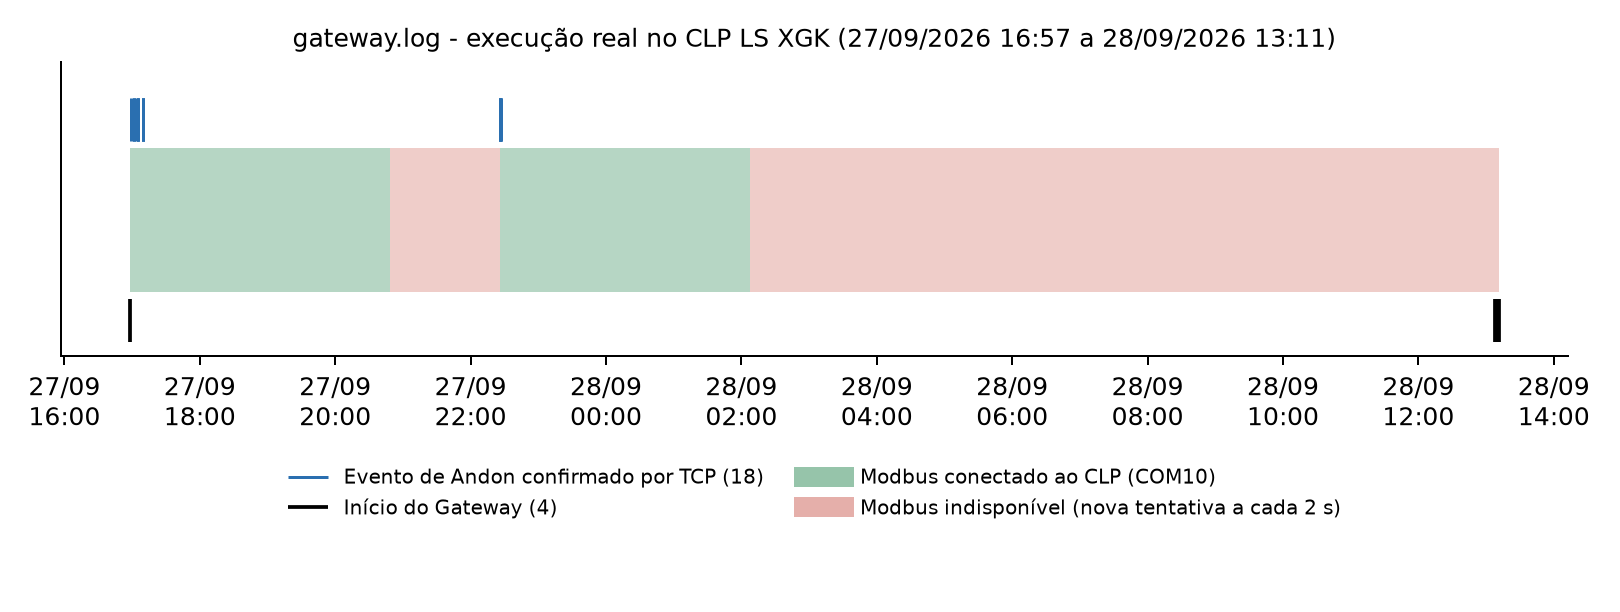
\includegraphics[width=1.00\textwidth]{Imagens/ev_linha_tempo_gateway_log.png}
    \caption{Linha do tempo da execução real: períodos com Modbus conectado (verde) e indisponível (vermelho), eventos confirmados e partidas do serviço. (arquivo: Imagens/ev\_linha\_tempo\_gateway\_log.png)}
    \label{fig:gwlog}
\end{figure}

A Figura \ref{fig:gwlog} mostra dois períodos de comunicação. O primeiro (16:57 a 20:48) concentra os eventos 1 a 12. Após a perda de comunicação de 20:48, o serviço não encerrou: manteve o OPC UA e o TCP ativos, tentou reabrir a porta a cada 2 s e, quando o adaptador voltou (22:26:21), retomou a leitura, entregou os quatro eventos retidos na FIFO do CLP (seção 3.5), sincronizou o relógio dois segundos depois e capturou os eventos 17 e 18. A segunda interrupção (02:07) não foi seguida de reconexão até o encerramento manual. Os 4.444 erros \cod{could not open port} são, portanto, a evidência do mecanismo de reconexão, e não falhas de processamento: nenhum evento foi perdido ou duplicado (18 capturados, 18 confirmados, \cod{attempts = 0}).

\subsection{Evidência: Gateway real contra o CLP emulado}\label{sec:emulado}

Para demonstrar os comandos de base, Start e reset e para capturar telas sem o hardware, o Gateway foi executado sem nenhuma alteração de código contra \cod{clp\_emulado.py}, um servidor Modbus RTU (biblioteca pymodbus) que expõe o mesmo mapa da Tabela \ref{tab:mapa} e imita o Ladder de forma simplificada: fila de eventos com o \textit{handshake} \cod{D100}/\cod{P10000}, aplicação do relógio por \cod{P10001}, base de tempos em \cod{D17001}, Start por \cod{P10002}, reset por \cod{P10003}, fluxo de uma peça por vez entre os 12 postos com os estados 0 a 3, contador \cod{D16052}, Andons em \cod{D109}-\cod{D111} e comando do motor em \cod{D112}. O Gateway apenas troca a porta serial por \cod{socket://127.0.0.1:5020}, recurso da própria pyserial; o protocolo continua sendo Modbus RTU, com CRC.

Na execução de 21/11/2026 (20:13 a 20:18), o Gateway \cod{LINHA\_DEMO}:
\begin{itemize}
    \item conectou-se, habilitou a leitura dos estados e do contador (\cod{process status available}, \cod{production count available}) e, sem servidor NTP disponível, aplicou a hora do sistema ao CLP uma única vez. O CLP emulado recebeu \cod{D1000}-\cod{D1003} = \cod{0x1126 0x2021 0x5313 0x2006}, isto é, 21/11/(20)26, 20:13:53, sábado (6) - codificação BCD correta;
    \item gravou e conferiu as 288 palavras da base (\cod{POST /api/process/cycle-base}, 5,3 s), pulsou \cod{P10002} e confirmou o Start quando o P01 chegou ao estado 2 (\cod{confirmed: true});
    \item capturou e entregou 6 eventos de Andon (P05 Equipamento, P09 Qualidade e P03 Material, ligado e desligado), com ACK no CLP entre 15,1 e 17,3 ms (mediana 15,9 ms) e entrega TCP entre 21,3 e 46,4 ms (mediana 23,1 ms), valores da mesma ordem dos medidos com o CLP real;
    \item executou o reset (\cod{P10003}, 2,7 s) e conferiu \cod{D16052 = 0}, e encerrou de forma ordenada pelo arquivo de parada.
\end{itemize}
